\documentclass[11pt,a4paper]{article}
\usepackage[margin=24mm]{geometry}
\usepackage{amsmath,amssymb,graphicx}
\title{Exercise 5.35(b): Otter--Dwass Formula}
\author{Statement and Comment: Russell Lyons and Yuval Peres\\Proof: Jim Pitman}
\date{Fixed paperback: August 19, 2026 \qquad TR 482: May 29, 1997}
\begin{document}
\maketitle
\section*{Original problem}
\noindent\emph{Lyons--Peres, physical page 188. The introductory definitions and part (b).}\par\medskip
\textbf{5.35.} Let $L$ be the offspring random variable of a Galton--Watson process. There are various useful ways to encode by a random walk the family tree when it is finite. We consider one such way here. Suppose that the process starts with $k$ individuals, that is, $Z_0=k$. Let $Z_{\mathrm{tot}}:=\sum_{n\ge 0}Z_n$ be the total size of the process. Let $S_n:=\sum_{j=1}^n(L_j-1)$, where $L_j$ are independent copies of $L$.

\textbf{(b) (Otter--Dwass Formula)} Show that $\mathbf{P}[Z_{\mathrm{tot}}=n]=\frac{k}{n}\mathbf{P}[S_n=-k]$.

\section*{Original Comment}
\noindent\emph{Lyons--Peres, physical page 630. This Comment is background.}\par\medskip
\textbf{5.35.} There are various ways to prove these; see Pitman (1998) for some of them and the history. For (a), one way to proceed is to replace the tree in stages as follows: replace the initial individuals by their progeny; then replace each of these in turn by their progeny; and so on. Each replacement decreases the total by a copy of $L-1$. For (b), given $L_j$ with $S_n=-k$, show that among the $n$ cyclic permutations of $\langle L_j;\ j\le n\rangle$, there are exactly $k$ for which the first time the sum is $-k$ is $n$ (that is, for which the event in (a) occurs). You might want to do this first for $k=1$.

\clearpage
\section*{Context for Pitman's proof}
\noindent\emph{TR 482, physical pages 2, 3, and 5--7. Selected definitions and theorem statements.}\par\medskip
\section*{1\quad Introduction}

Let $(Z_0,Z_1,\ldots)$ be a \emph{Galton-Watson branching process with offspring distribution} $(p_i;\ i=0,1,\ldots)$, where $p_i\ge 0$, $\sum_i p_i=1$. Interpret $p_i$ as the probability that an individual has $i$ children, and $Z_g$ as the number of individuals in the $g$th generation of a population starting from some initial number $Z_0$. For each $g\ge 0$, it is assumed that given the evolution of the population up to the $g$th generation, the $Z_g$ individuals in the $g$th generation have independent random numbers of children distributed according to $(p_i)$. These children are the $Z_g$ members of the $(g+1)$th generation. See [30, 33, 5] for background.

Let
\[
S_n:=X_1+\cdots+X_n \tag{1}
\]
be the sum of $n$ independent random variables $X_j$ with common distribution $(p_i)$. From the description of $(Z_0,Z_1,\ldots)$, this sequence is a Markov chain with state space $\{0,1,2,\ldots\}$ and time-homogeneous transition probabilities
\[
P(Z_{g+1}=m\mid Z_g=n)=P(S_n=m) \tag{2}
\]
where for each $n$ the sequence $(P(S_n=m),\ m=0,1,\ldots)$ is the $n$-fold convolution of the sequence $(p_i;\ i=0,1,\ldots)$ with itself. Two elementary expressions for $P(S_n=m)$ in terms of $(p_i)$ are recalled in formulae (7) and (8) below. Let
\[
\#\mathcal{F}_k:=\sum_{g=0}^{\infty} Z_g\in\{1,2,\ldots,\infty\} \tag{3}
\]
represent the \emph{total progeny} in the branching process given $Z_0=k$ individuals to start with. Here $\#\mathcal{F}_k$ stands for the number of individuals in the random family $\mathcal{F}_k$ generated by the branching process. In Section 4, $\mathcal{F}_k$ will be defined as a \emph{random family forest}, that is a collection of $k$ \emph{random family trees}, one for each of the $k$ initial individuals. The following theorem presents a remarkable formula for the distribution of $\#\mathcal{F}_k$ restricted to positive integers. This formula was discovered by Otter [43] for $k=1$ and extended to all $k\ge 1$ by Dwass [17]:

\textbf{Theorem 1} (Otter-Dwass formula) \emph{For all $n,k=1,2,\ldots$}
\[
P(\#\mathcal{F}_k=n)=\frac{k}{n}P(S_n=n-k). \tag{4}
\]

The first approach to these formulae was by the method of probability generating functions. Let
\[
g(z):=\sum_{i=0}^{\infty} p_i z^i \tag{6}
\]
be the probability generating function derived from the offspring distribution $(p_i)$. Two elementary expressions for $P(S_n=m)$ are
\begin{align}
P(S_n=m)&=\text{coefficient of } z^m \text{ in } g(z)^n \tag{7}\\
&=\sum_{\substack{\Sigma n_i=n\\ \Sigma i n_i=m}} \binom{n}{n_0,\ldots,n_n}\prod_{i\ge 0} p_i^{n_i} \tag{8}
\end{align}
where the sum ranges over the finite set of all sequences of non-negative integers $(n_i,i\ge 0)$ with $\Sigma n_i=n$ and $\Sigma i n_i=m$. Here
\[
\binom{n}{n_0,\ldots,n_n}:=\frac{n!}{n_0!\cdots n_n!} \tag{9}
\]
is the multinomial coefficient which is the number of sequences $(i_j,1\le j\le n)$ of \emph{type} $(n_i,i\ge 0)$, that is sequences $(i_j)$ such that $\#\{j: i_j=i\}=n_i$ for all $i\ge 0$ and hence $\sum_j i_j=\sum_i i n_i$.

The term \emph{forest} will be used here for a \emph{finite rooted forest}, that is a directed graph with a finite number of vertices, each of whose connected components is a tree with edges directed away from its root vertex. A forest with vertex set $V$ is said to be \emph{labeled by $V$}. For vertices $v$ and $w$ of a forest $\mathbf{f}$ write $v\xrightarrow{\mathbf{f}} w$ to show that $(v,w)$ is a directed edge of $\mathbf{f}$. The \emph{number of children} or \emph{out-degree} $v$ in the forest $\mathbf{f}$ is $C(v,\mathbf{f}):=\#\{w: v\xrightarrow{\mathbf{f}} w\}$. In a \emph{plane forest} $\mathbf{f}$ with $k$ component trees, the set of roots of the tree components is ordered, as is the set of children of $v$ for each vertex $v$ of $\mathbf{f}$. Regard a plane forest with $k$ root vertices as a collection of family trees, one for each of $k$ initial individuals, with each vertex in the forest corresponding to an individual, and with the order of the roots and the orders of children corresponding to the order of birth of individuals. A plane forest is often depicted without labels as on the left side of Figure 1, and called an \emph{unlabeled plane forest}. However, there is a natural way to identify each vertex of a plane forest by a finite sequence of non-negative integers which indicates the location of the vertex in the forest. So, following the convention of [30] for labeling family trees, the set of vertices of a plane forest will be identified as a subset of the set of all finite sequences of integers, as illustrated on the right side of Figure 1.

\begin{center}
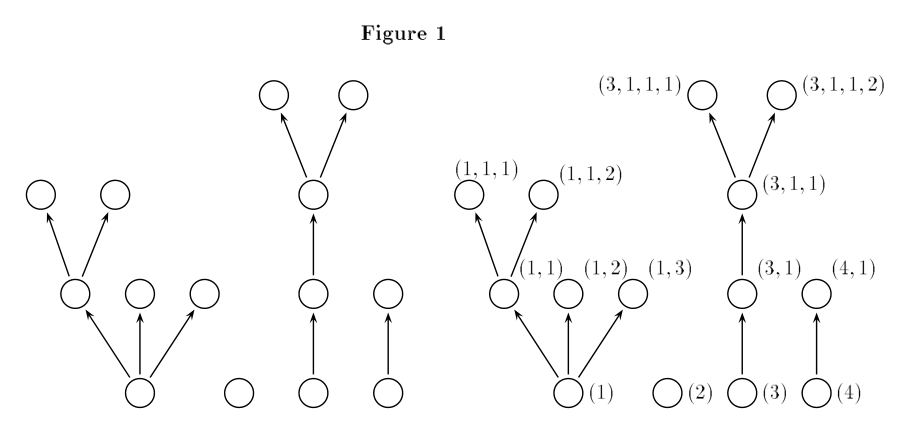
\includegraphics[width=\linewidth]{figures/pitman-tr482-figure-1.png}
\end{center}

An individual in the $g$th generation of a family forest (= vertex at height $g$ in the plane forest) is identified by a sequence of $g+1$ integers, for instance $(3,7,4)$ to indicate a second generation individual who is the 4th child of the 7th child of the 3rd root individual.

The \emph{type} of a forest $\mathbf{f}$ is the sequence of non-negative integers $(n_i)$, where $n_i$ is the number of vertices of $\mathbf{f}$ with $i$ children. Let $1\le k\le n$ and let $(n_i)$ be a sequence of non-negative integers with
\[
\sum_i n_i=n\quad\text{and}\quad \sum_i i n_i=n-k. \tag{12}
\]
A forest of type $(n_i)$ has $n$ vertices and $n-k$ non-root vertices, hence $k$ root vertices and $k$ tree components.

\textbf{Theorem 4} (Enumeration of plane forests by type) [18, 19, 43, 54] \emph{For $1\le k\le n$ and $(n_i)$ subject to (12) the number $N^{\mathit{plane}}(n_0,n_1,\ldots)$ of plane forests of type $(n_i)$ with $k$ tree components and $n$ vertices is}
\[
N^{\mathit{plane}}(n_0,n_1,\ldots)=\frac{k}{n}\binom{n}{n_0,\ldots,n_n}. \tag{13}
\]

\textbf{Theorem 5} (Enumeration of labeled forests by type) [59, Cor.\ 3.5] \emph{Let $[n]:=\{1,\ldots,n\}$. For $1\le k\le n$ and $(n_i)$ subject to (12), the number $N^{[n]}(n_0,n_1,\ldots)$ of forests labeled by $[n]$ of type $(n_i)$ with $k$ tree components and $n$ vertices is}
\[
N^{[n]}(n_0,n_1,\ldots)=\frac{k}{n}\binom{n}{k}\frac{(n-k)!}{\prod_{i\ge 0}(i!)^{n_i}}\binom{n}{n_0,\ldots,n_n}. \tag{14}
\]

The enumeration of plane forests by type is simpler than its companion for labeled forests. But the result for labeled forests has the following simpler equivalent:

\textbf{Theorem 6} (Enumeration of labeled forests by out-degree sequence) [51],[59, Thm.\ 3.4] \emph{For all sequences of non-negative integers $(c_1,\ldots,c_n)$ with $\sum_i c_i=n-k$ the number $N(c_1,\ldots,c_n)$ of forests $\mathbf{f}$ with vertex set $[n]$ in which vertex $i$ has $c_i$ children for each $i\in[n]$ (and hence $\mathbf{f}$ has $k$ tree components) is}
\[
N(c_1,\ldots,c_n)=\frac{k}{n}\binom{n}{k}\binom{n-k}{c_1,\ldots,c_n}. \tag{15}
\]

\medskip
\noindent\emph{Author's notation excerpt immediately after (16).}\par\smallskip
where the sum is over the set $\mathbf{F}_{k,n}$ of all forests with $k$ tree components labeled by $[n]$, and $C(i,\mathbf{f})$ is the number of children of $i$ in the forest $\mathbf{f}$.

\clearpage
\section*{Original proof}
\noindent\emph{TR 482, physical pages 9--12. The proof in Sections 2--4, through the equivalence of Theorems 1 and 4.}\par\medskip
\section*{2\quad Enumeration of labeled forests by out-degree sequence.}

\noindent\textbf{Proof of Theorem 6.} For a forest $\mathbf{f}$ with vertex set $[n]$ and $i\in[n]$ let $J_i(\mathbf{f}):=\{j\in[n]: i\xrightarrow{\mathbf{f}} j\}$ be the set of children of $i$ in $\mathbf{f}$. So $\mathbf{f}$ is determined by the sequence of disjoint sets $J_1(\mathbf{f}),\ldots,J_n(\mathbf{f})$, and vice-versa. Given a sequence of disjoint subsets $J_1,\ldots,J_n$ of $[n]$, for each $m\in[n]$ let $\mathbf{f}_m$ be the relation on $[m]\cup(\bigcup_{i=1}^m J_i)$ defined by
\[
i\xrightarrow{\mathbf{f}_m} j \quad\text{iff}\quad i\in[m]\text{ and } j\in J_i. \tag{19}
\]
There exists a forest $\mathbf{f}$ labeled by $[n]$ such that $J_i(\mathbf{f})=J_i$ for all $i\in[n]$ if and only if the $J_i$ are such that $\mathbf{f}_m$ defined by (19) is a forest with vertex set $[m]\cup(\bigcup_{i=1}^m J_i)$ for every $m\in[n]$; then $\mathbf{f}=\mathbf{f}_n$ and $\mathbf{f}_m$ is the restriction of $\mathbf{f}$ to $[m]\cup(\bigcup_{i=1}^m J_i)$ for each $m\in[n]$. It follows that for each sequence of non-negative integers $(c_i)$ with $\sum_i c_i=n-k$, the number
\[
N(c_1,\ldots,c_n):=\#\{\mathbf{f}\in\mathbf{F}_{k,n}: \#J_i(\mathbf{f})=c_i \text{ for all } i\in[n]\} \tag{20}
\]
is the number of ways to choose a sequence of subsets $(J_1,\ldots,J_n)$ of $[n]$ such that $\#J_m=c_m$ and the relation $\mathbf{f}_m$ defined by (19) is a forest with vertex set $[m]\cup(\bigcup_{i=1}^m J_i)$ for every $m\in[n]$. Clearly, $J_1$ can be any of the $\binom{n-1}{c_1}$ subsets of $[n]-\{1\}$ of size $c_1$. For $m\in[n-1]$ make the inductive hypothesis that sets $J_1,\ldots,J_m$ of sizes $c_1,\ldots,c_m$ have been chosen so that $\mathbf{f}_m$ is a forest. Which choices of $J_{m+1}$ of size $c_{m+1}$ make $\mathbf{f}_{m+1}$ a forest? There are two cases to consider. Either

(i) $m+1\notin\bigcup_{i=1}^m J_i$: then $J_{m+1}$ can be any subset of $[n]-(\bigcup_{i=1}^m J_i)-\{m+1\}$;

or

(ii) $m+1\in\bigcup_{i=1}^m J_i$: then $J_{m+1}$ can be any subset of $[n]-(\bigcup_{i=1}^m J_i)-\{r_m\}$ where $r_m\notin\bigcup_{i=1}^m J_i$ is the root of the tree component of $\mathbf{f}_m$ which contains $m+1$. Either way, and regardless of what sets $J_1,\ldots,J_m$ of sizes $c_1,\ldots,c_m$ were previously chosen to make $\mathbf{f}_m$ a forest, the number of possible choices of $J_{m+1}$ which make $\mathbf{f}_{m+1}$ a forest is
\[
\binom{n-\sum_{i=1}^m c_i-1}{c_{m+1}}.
\]

Consequently, by induction
\[
N(c_1,\ldots,c_n)=\binom{n-1}{c_1}\binom{n-c_1-1}{c_2}\cdots\binom{n-\sum_{i=1}^{n-1}c_i-1}{c_n}
\]
and this expression simplifies easily to yield (15). \hfill$\square$

\section*{3\quad Enumeration of forests by type}

\noindent\textbf{Proof of Theorem 5.} Let $(n_i)$ subject to (12) be a possible type sequence for a forest of $k$ trees with $n$ vertices. According Theorem 6, for each particular sequence $(c_j)$ of type $(n_i)$ the number of forests in which $j$ has $c_j$ children for all $j\in[n]$ is
\[
\frac{k}{n}\binom{n}{k}\frac{(n-k)!}{c_1!\cdots c_n!}=\frac{k}{n}\binom{n}{k}\frac{(n-k)!}{\prod_{i\ge 0}(i!)^{n_i}}. \tag{21}
\]
But the number of sequences of non-negative integers $(c_j)$ such that $(c_j)$ has type $(n_i)$ is just the multinomial coefficient (9). The number of forests labeled by $[n]$ of type $(n_i)$ is the product of the number in (21) and this multinomial coefficient. Thus Theorem 6 implies Theorem 5, and vice versa. \hfill$\square$

\noindent\textbf{Proof of Theorem 4.} The enumeration (13) for plane forests corresponds to the enumeration (14) for labeled forests via the following map $\Psi$, which transforms a forest $\mathbf{f}$ labeled by $[n]$ into a plane forest $\Psi(\mathbf{f})$ of the same type. To define $\Psi(\mathbf{f})$, first place the components of $\mathbf{f}$ in order of their root labels, then recursively for each $g\ge 0$ place the children of each vertex of $\mathbf{f}$ at height $g$ in order of their labels. Finally, delabel to obtain the plane forest $\Psi(\mathbf{f})$. See Figure 2.

\begin{center}
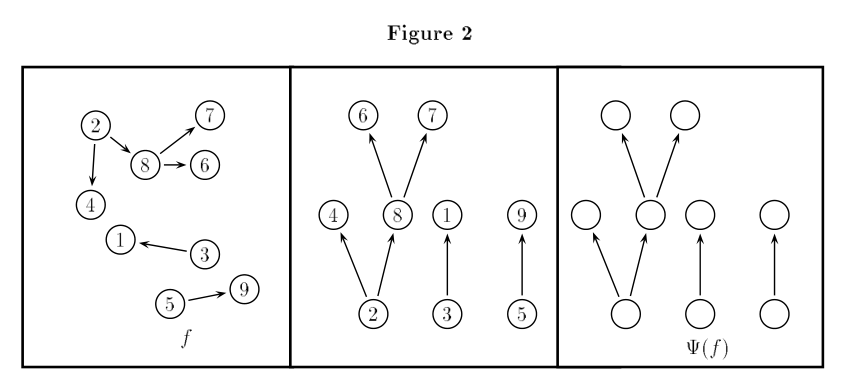
\includegraphics[width=\linewidth]{figures/pitman-tr482-figure-2.png}
\end{center}

For a fixed plane forest $\mathbf{f}^{\circ}$ with $n$ vertices and $k$ root vertices, and type $(n_i)$, let $\{v_1,\ldots,v_n\}$ be a listing of the vertices in some arbitrary order. Let $B_0$ be the set of roots of $\mathbf{f}^{\circ}$, and $B_i$ the set of children of $v_i$ for $i=1,\ldots,n$. The sets $B_i$, $0\le i\le n$, some of which must be empty, are disjoint with union $V(\mathbf{f}^{\circ})$, the set of vertices of $\mathbf{f}^{\circ}$. As discussed earlier, $V(\mathbf{f}^{\circ})$ is regarded as a subset of the set of finite sequences of positive integers. Each non-empty $B_i$ has a linear ordering, and each $\mathbf{f}\in\Psi^{-1}(\mathbf{f}^{\circ})$ corresponds to a unique bijection from $V(\mathbf{f}^{\circ})$ to $[n]$ which is increasing on each non-empty $B_i$. It follows that $\#\Psi^{-1}(\mathbf{f}^{\circ})$, the number of forests $\mathbf{f}$ labeled by $[n]$ such that $\Psi(\mathbf{f})=\mathbf{f}^{\circ}$ is the multinomial coefficient
\[
\#\Psi^{-1}(\mathbf{f}^{\circ})=\binom{n!}{k,\#B_1,\ldots,\#B_n}=\frac{n!}{k!\prod_{v\in V(\mathbf{f}^{\circ})} C(v,\mathbf{f}^{\circ})!}=\frac{n!}{k!\prod_{i\ge 0}(i!)^{n_i}} \tag{22}
\]
where $C(v,\mathbf{f}^{\circ})$ is the number of children of $v$ in the forest $\mathbf{f}^{\circ}$, and $(n_i)$ is the type of $\mathbf{f}^{\circ}$ and of every $\mathbf{f}\in\Psi^{-1}(\mathbf{f}^{\circ})$. It follows that the number $N^{\mathit{plane}}(n_0,n_1,\ldots)$ of plane forests of type $(n_i)$ and the corresponding number $N^{[n]}(n_0,n_1,\ldots)$ of forests of type $(n_i)$ labeled by $[n]$ are related by
\[
\frac{N^{[n]}(n_0,n_1,\ldots)}{N^{\mathit{plane}}(n_0,n_1,\ldots)}=\frac{n!}{k!\prod_{i\ge 0}(i!)^{n_i}}. \tag{23}
\]
Hence the equivalence of Theorems 4 and 5. \hfill$\square$

\section*{4\quad The Otter-Dwass formula}

\noindent\textbf{Proof of the equivalence of Theorems 1 and 4.} Following Otter [43] and subsequent authors [30, 37, 13], regard a Galton-Watson process started with $Z_0=k$ individuals as generating a collection of $k$ family trees, which combine to form a random family forest $\mathcal{F}_k$. On the event $(\#\mathcal{F}_k<\infty)$ the random family forest $\mathcal{F}_k$ can be defined in an elementary way as a random element with values in the countable set $\mathbf{F}$ of all plane forests. The distribution of $\mathcal{F}_k$ is then the sub-probability distribution on $\mathbf{F}$ defined by the formula [43]
\[
P(\mathcal{F}_k=\mathbf{f})=\prod_{v\in V(\mathbf{f})} p_{C(v,\mathbf{f})}=\prod_{i\ge 0} p_i^{n_i(\mathbf{f})} \quad \forall k\ge 1,\ \mathbf{f}\in\mathbf{F}_k^{\mathit{plane}} \tag{24}
\]
where $V(\mathbf{f})$ is the set of vertices of $\mathbf{f}$, the number of vertices of $\mathbf{f}$ with $i$ children is denoted $n_i(\mathbf{f})$, and $\mathbf{F}_k^{\mathit{plane}}$ is the set of plane forests with $k$ root vertices. This distribution on $\mathbf{F}_k^{\mathit{plane}}$ has total mass $P(\#\mathcal{F}_k<\infty)\le 1$. For each $k=1,2,\ldots$ the probability of the event $(\#\mathcal{F}_k=n)$ is obtained by summing the expression (24) over all plane forests $\mathbf{f}$ of $k$ trees with a total of $n$ vertices. The terms in this sum can be classified by the type $(n_i)$ of the forest $\mathbf{f}$. Since the number of vertices in a forest of type $(n_i)$ is $\sum_i n_i$ and the number of root vertices is $n-\sum_i n_i$, the result is
\[
P(\#\mathcal{F}_k=n)=\sum_{\substack{\Sigma n_i=n\\ \Sigma i n_i=n-k}} N^{\mathit{plane}}(n_0,n_1,\ldots)\prod_{i\ge 0} p_i^{n_i} \tag{25}
\]
where the sum is over all possible types of a sequence with length $n$ and sum $n-k$. Now fix $n$ and $k$ and regard the probability displayed in (25), and the probability $P(S_n=m)$ displayed in (8) for $m=n-k$, as functions of the sequence $(p_0,\ldots,p_n)$. Since each probability is a polynomial in $(p_0,\ldots,p_n)$, the Otter-Dwass formula (4) is an identity of polynomials whose coefficient identity is the enumeration (13) of plane forests by type. \hfill$\square$

\section*{Source notes}
\noindent This reading transcription uses the fixed 1997 author PostScript, read through its existing mechanical PDF conversion.\\[3pt]
\noindent Equation (22) retains the printed $n!$ at the top of the first multinomial. Compare the original definition (9) and the factorial ratios printed in (22).\\[3pt]
\noindent The root count sentence before (25) is reproduced as printed. The type constraints in (12) and (25) state $\sum_i i n_i=n-k$.
\end{document}
